阿恩特(Fritz Georg Arndt,1885.7.6--1969.12.8)是一位对土耳其的化学发展有着重要影响的德国化学家。在他的职业生涯中,他在土耳其伊斯坦布尔大学工作了二十余年。他和艾司特(Bernd Eistert)一同发现了阿恩特-艾司特合成法。这种合成法是一个可让羧酸碳链增长一个碳原子的反应,从而被称为同系增碳过程。在阿恩特-艾司特同系增碳反应中,关键的一步是利用沃尔夫重排(Wolff Rearrangement),在光照、加热或银(Ⅰ)盐催化下将重氮酮转化为烯酮。在亲核试剂如水、醇或胺的存在下,烯酮中间体会反应生成相应的羧酸、酯或酰胺。在本题中,我们会研究吲哚里西啶类生物碱的合成。

\begin{figure}[h]
	\centering
	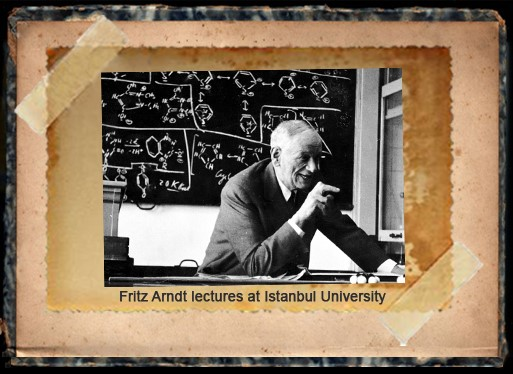
\includegraphics[width=10cm]{./pic/t5-1.jpg}
\end{figure}

根据以上描述,吲哚里西啶167B和去氢毒芹碱的合成易于通过$\beta$,$\gamma$-不饱和酯\textbf{B}实现。其关键的步骤\textbf{A}$\rightarrow$\textbf{B}是一步沃尔夫重排。化合物\textbf{C}含有内酰胺结构,且是一个包含六元环与饱和五元环稠合结构的双环杂环化合物,其中的一个桥头原子是氮原子。

\noindent\textbf{5.1.} 请画出\textbf{A-D}的机构(不需表示立体化学)。

\begin{figure}[h]
	\centering
	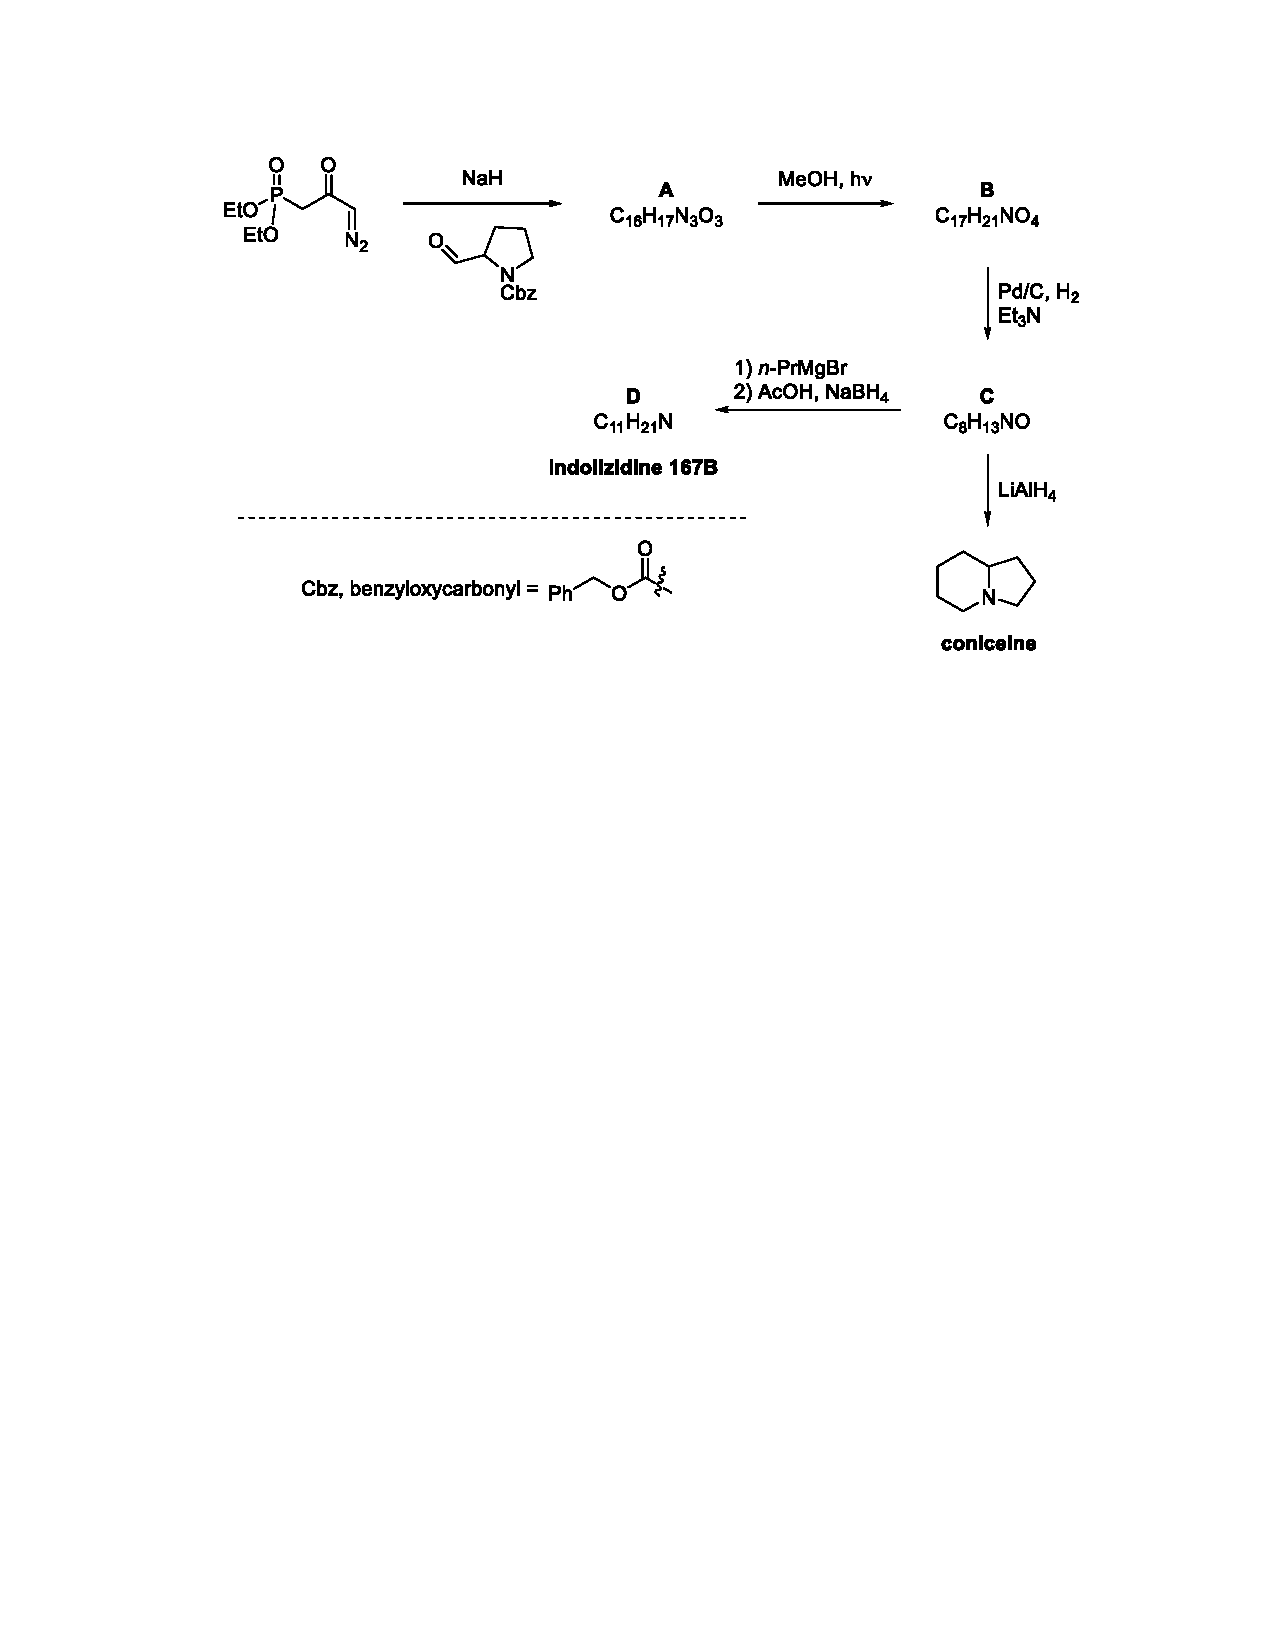
\includegraphics[width=14cm]{./pic/t5-2.pdf}
\end{figure}

在阿恩特-艾司特同系增碳反应中,$\alpha$-重氮酮可以通过光引发的沃尔夫重排转化为α-羰基卡宾,并伴随着氮气的生成。这个中间体会经历一个1,2-烷基迁移从而给出烯酮产物。

\noindent\textbf{5.2.}
画出在第二步\textbf{A}$\rightarrow$\textbf{B}中$\alpha$-羰基卡宾和烯酮中间体的结构。

以丙基溴化镁对化合物\textbf{C}进行加成,随后以AcOH/NaBH\textsubscript{4}处理,是吲哚里西啶167B全合成的最后一步。

\noindent\textbf{5.3.}
画出在第四步\textbf{C}$\rightarrow$\textbf{D}中中间体C\textsubscript{11}H\textsubscript{20}N\textsuperscript{+}的结构。

\noindent\textbf{5.4.}
去氢毒芹碱的另一个合成方法描述如下。画出化合物\textbf{E}-\textbf{J}的结构。

\begin{figure}[h]
	\centering
	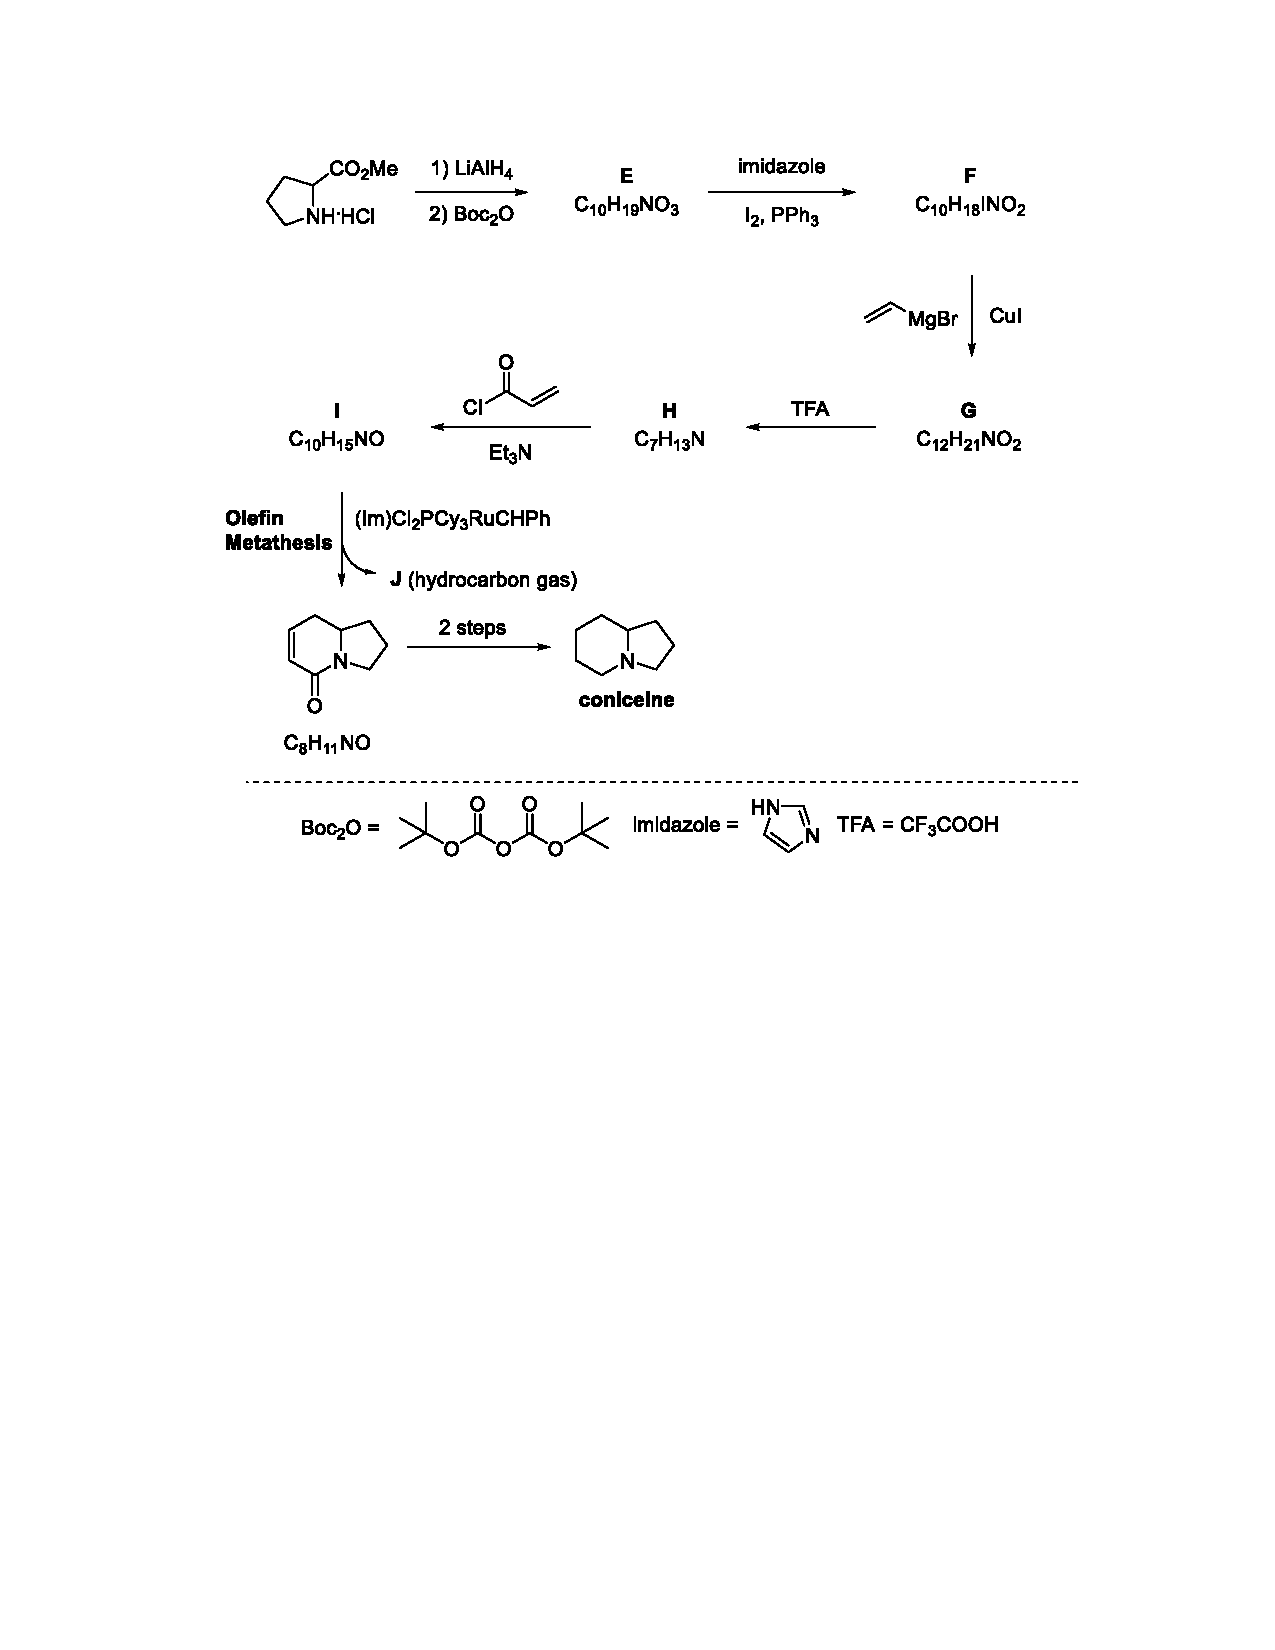
\includegraphics[width=14cm]{./pic/t5-3.pdf}
\end{figure}

